\documentclass{beamer}

% Thème sobre et académique
\usetheme{Madrid}
\usecolortheme{seahorse}

% Langue et encodage
\usepackage[utf8]{inputenc}
\usepackage[french]{babel}
\usepackage{lmodern}
\usepackage{booktabs}


% Couleur personnalisée
\definecolor{c}{RGB}{120,20,30}
\setbeamercolor{title}{fg=white,bg=c}
\setbeamercolor{frametitle}{fg=white,bg=c}
\setbeamercolor{structure}{fg=c}

% Informations de la présentation
\title[Apprentissage de classes déséquilibrées]{\textbf{Apprentissage de classes déséquilibrées}}
\subtitle{\LARGE HAX907X - Apprentissage statistique}
\author[]{\textbf{SAWADOGO Kader \\ GERMAIN Marine \\ LABOURAIL Célia \\ MARIAC Damien}}
\institute[Université Montpellier]{Université Montpellier \\ Département de Mathématique}
\date{\today}

\AtBeginSection[]
{
  \begin{frame}{Sommaire}
    \tableofcontents[currentsection]
  \end{frame}
}

\begin{document}



\begin{frame}
  \titlepage
\end{frame}
\section{Contexte}

\begin{frame}{Problème du déséquilibre et motivation du projet}
\small

\begin{block}{Un jeu de données très déséquilibré}
\begin{itemize}
    \item   CréditCard  : \textbf{284\,807 transactions}, dont seulement \textbf{492 fraudes} (\textbf{0,17\,\%}).
    \item $\Rightarrow$ Les modèles ont tendance à ignorer la classe minoritaire.
\end{itemize}
\end{block}

\vspace{0.3cm}

\begin{block}{Illustration du problème}
\centering
\begin{tabular}{lccc}
\toprule
\textbf{Modèle} & \textbf{Recall} & \textbf{Precision} & \textbf{F1-score} \\
\midrule
Régression Logistique & 0.59 & 0.89 & 0.70 \\
Random Forest (200 arbres) & 0.60 & 0.95 & 0.85 \\
\bottomrule
\end{tabular}
\end{block}

\end{frame}

\section{Problématique}

\begin{frame}{Problématique scientifique}
    \centering
    \Large{Comment atténuer le déséquilibre des classes pour améliorer la performance réelle du modèle ?}
\end{frame}


\section{Méthodes}

\begin{frame}{Random Over-Sampling}
\begin{figure}
    \centering
    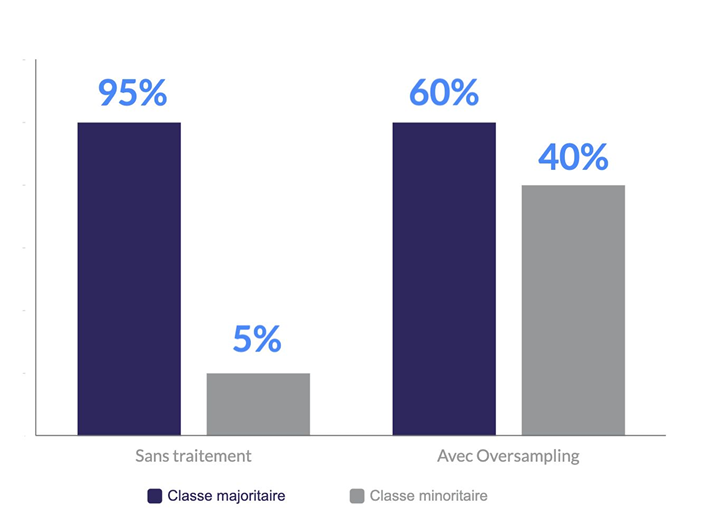
\includegraphics[width=0.95\textwidth]{images/ROS.png}
\end{figure}
    
\end{frame}

\begin{frame}
\begin{table}
\centering
\caption{Jeu de données après sur-échantillonnage (ROS )}
\begin{tabular}{|c|c|c|}
\hline
\textbf{x} & \textbf{label} & \textbf{source} \\ 
\hline
1   & 0 & original \\
2 &  0 & original \\
3 &  0 & original \\
4 &  0 & original \\
5 &  0 & original \\
6 &  0 & original \\
7 &  0 & original \\
8 &  1 & original \\
9 &  1 & original \\
10 &  1 & original \\
8 &  1 & dupliqué \\
 9 &  1 & dupliqué \\
 10 &  1 & dupliqué \\
 8 &  1 & dupliqué \\
\hline
\end{tabular}
\end{table}

\end{frame}

\begin{frame}{Random Under-Sampling}
\begin{figure}
    \centering
    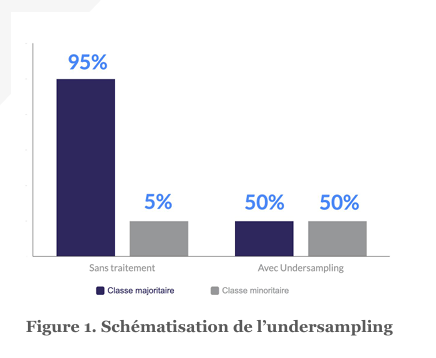
\includegraphics[width=0.95\textwidth]{images/RUS.png}

\end{figure}
\end{frame}

\begin{frame}
\begin{table}
\centering
\caption{Jeu de données après sous-échantillonnage (RUS)}
\begin{tabular}{|c|c|c|}
\hline
\textbf{x} & \textbf{label} & \textbf{source} \\ 
\hline
1   & 0 & supprimé\\
2 &  0 & supprimé \\
3 &  0 & supprimé \\
4 &  0 & original \\
5 &  0 & original \\
6 &  0 & original \\
7 &  0 & original \\
8 &  1 & original \\
9 &  1 & original \\
10 &  1 & original \\

\hline
\end{tabular}
\end{table}
\end{frame}

\begin{frame}
  \frametitle{SMOTE : Synthetic Minority Over-sampling Technique}
  \begin{figure}
      \centering
      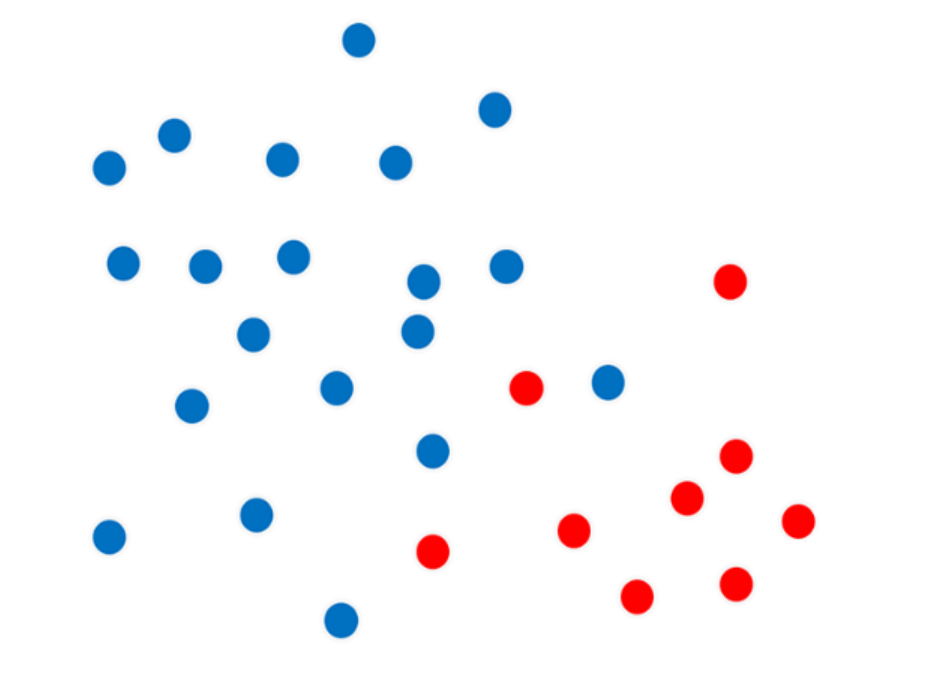
\includegraphics[width=0.7\textwidth]{images/SMOTEE.png}
      \caption{Schéma de SMOTE}
  \end{figure}

  \end{frame}

  \begin{frame}
      \frametitle{SMOTE : Synthetic Minority Over-sampling Technique}



      \begin{figure}
          \centering
          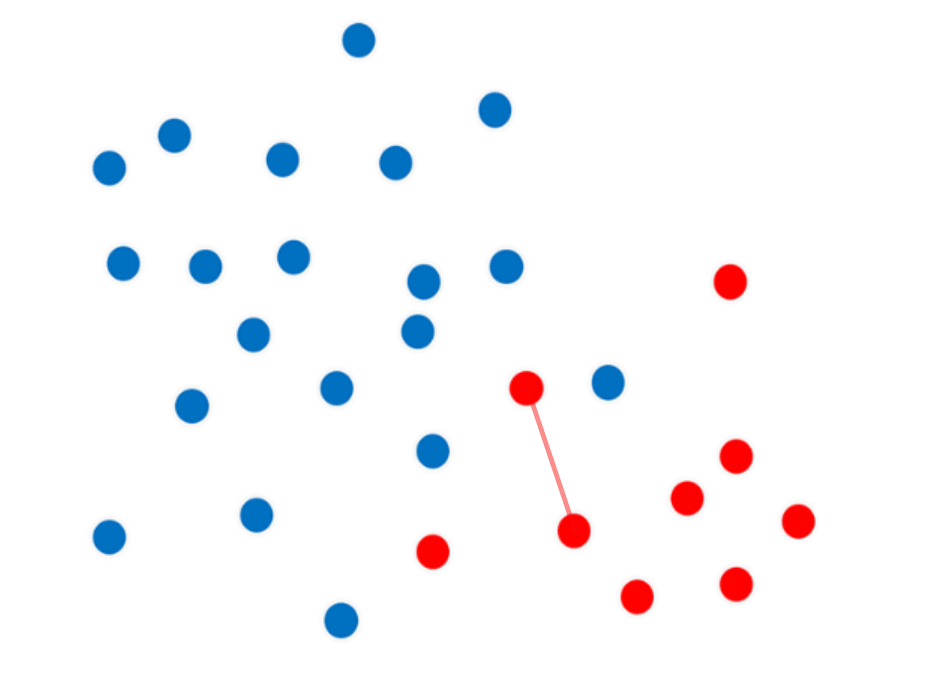
\includegraphics[width=0.7\textwidth]{images/SMOTED.png}
          \caption{Schéma de SMOTE}
      \end{figure}

  \end{frame}

  \begin{frame}
      \frametitle{SMOTE : Synthetic Minority Over-sampling Technique}

      \begin{figure}
          \centering
          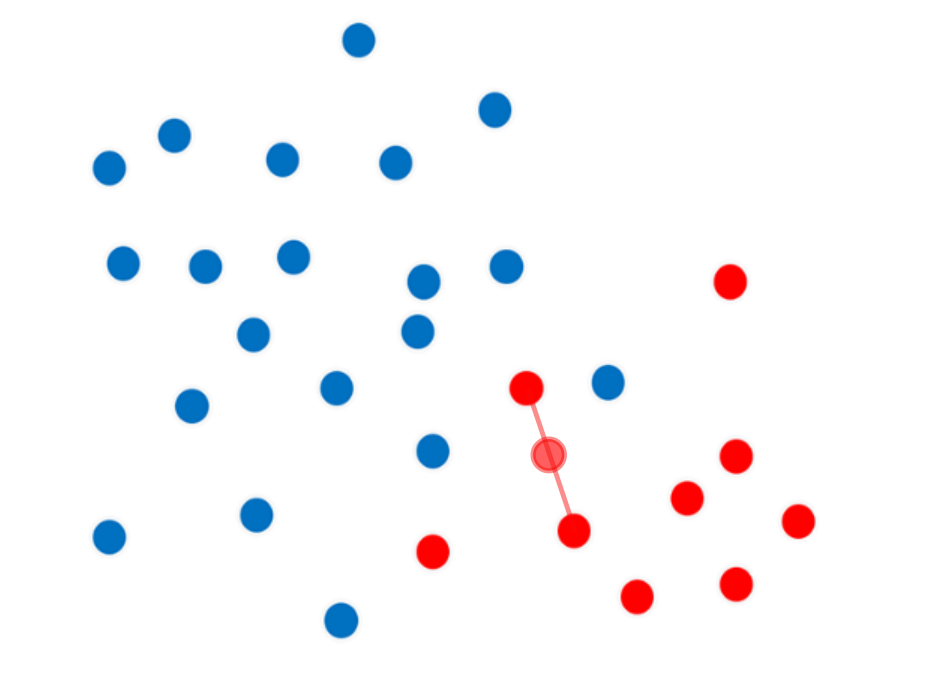
\includegraphics[width=0.7\textwidth]{images/SMOTEC.png}
          \caption{Schéma de SMOTE}
      \end{figure}

  \end{frame}

  \begin{frame}
      \frametitle{SMOTE : Synthetic Minority Over-sampling Technique}



      \begin{figure}
          \centering
          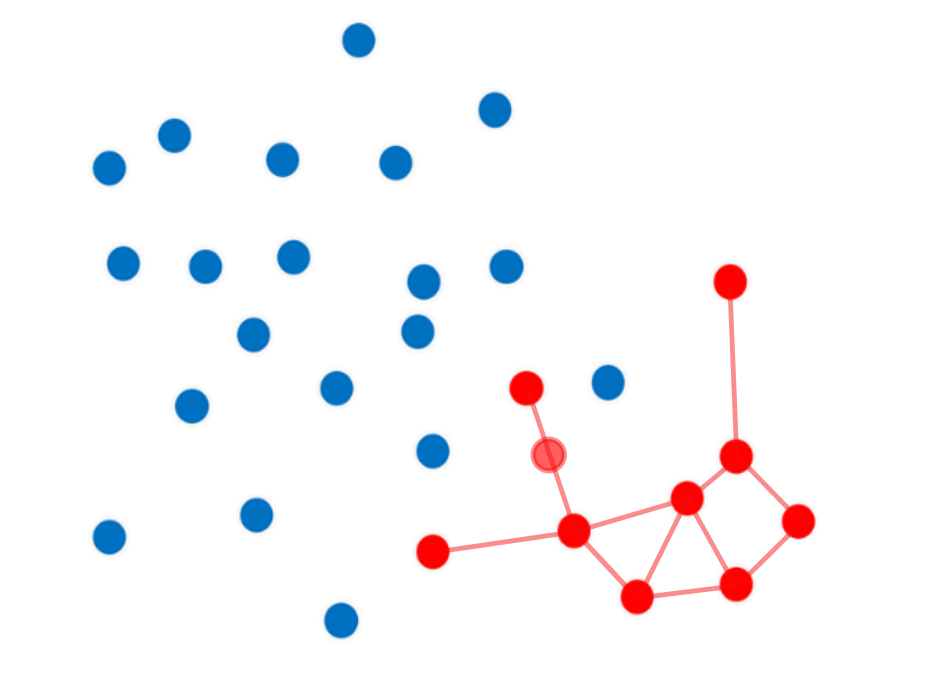
\includegraphics[width=0.7\textwidth]{images/SMOTEB.png}
          \caption{Schéma de SMOTE}
      \end{figure}

  \end{frame}

  \begin{frame}
      \frametitle{SMOTE : Synthetic Minority Over-sampling Technique}



      \begin{figure}
          \centering
          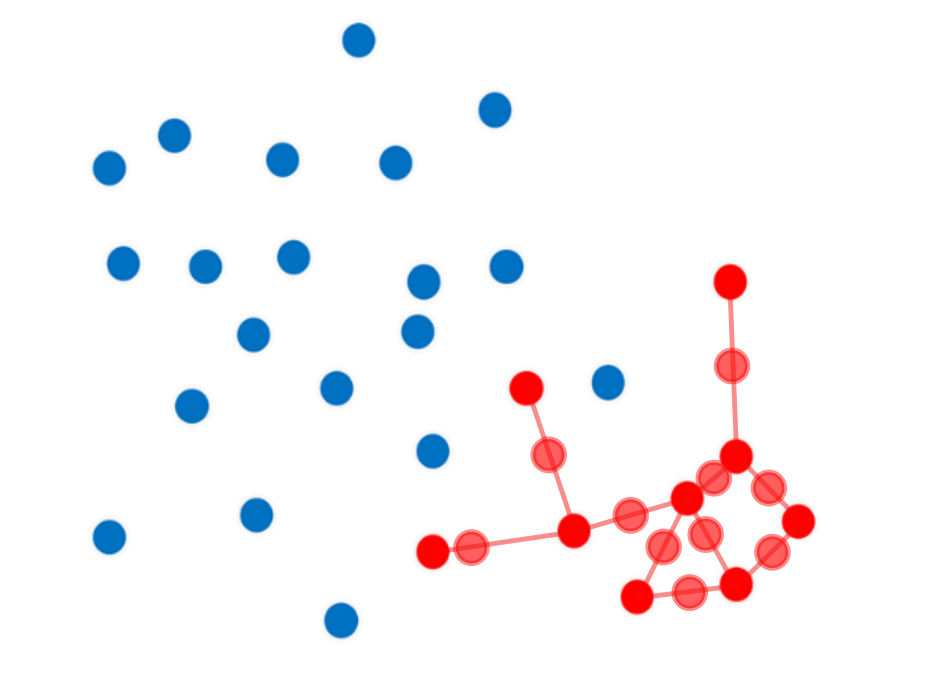
\includegraphics[width=0.7\textwidth]{images/SMOTEA.png}
          \caption{Schéma de SMOTE}
      \end{figure}

  \end{frame}






  \begin{frame}[t,shrink=8]{SMOTE : Synthetic Minority Over-sampling Technique}

    \begin{block}{Notations}
    \footnotesize
    \begin{columns}[T,totalwidth=\textwidth]
      \column{0.52\textwidth}
      \begin{itemize}
        \setlength{\itemsep}{1pt}\setlength{\parskip}{0pt}
        \item $n$ : nb \textbf{total} d'observations
        \item $n_{\min}$ : nb d'observations \textbf{minoritaires}
        \item $d$ : dimension (nb de variables)
      \end{itemize}
      \column{0.48\textwidth}
      \begin{itemize}
        \setlength{\itemsep}{1pt}\setlength{\parskip}{0pt}
        \item $k$ : nb de plus proches voisins
        \item $M$ : nb de points synthétiques générés
      \end{itemize}
    \end{columns}
    \end{block}

    \begin{block}{Étapes dominantes \& complexité (naïf)}
    \footnotesize
    \begin{enumerate}
      \setlength{\itemsep}{2pt}\setlength{\parskip}{0pt}
      \item \textbf{Recherche des $k$-PPV (vers tous les points)} :
            coût d'une distance $\mathcal O(d)$ $\Rightarrow$
            comparaison à $n$ points $\mathcal O(n\,d)$ $\Rightarrow$
            pour $n_{\min}$ points minoritaires $\boxed{\mathcal O(n_{\min}\,n\,d)}$.
      \item \textbf{Génération} :
            $x_{\text{new}} = x_i + \lambda(x_j-x_i)$, $\lambda\sim\mathcal U(0,1)$
            \hfill $\boxed{\mathcal O(M\,d)}$
    \end{enumerate}
    \end{block}

    \begin{block}{Synthèse}
    \footnotesize
    \[
    \boxed{T_{\text{SMOTE}}=\mathcal O(n_{\min}\,n\,d) + \mathcal O(M\,d)}
    \quad\text{(recherche kNN dominante).}
    \]
    \end{block}

  \end{frame}

\section{Limites des méthodes}

\begin{frame}{Limites des méthodes}
\begin{block}{ROS}
    \begin{itemize}
       \item Overfitting
   \end{itemize} 
\end{block}
    \begin{figure}
    \centering
    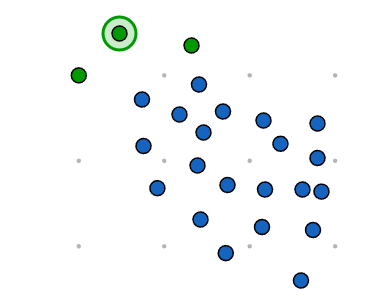
\includegraphics[width=0.7\textwidth]{images/lROS.png}
     
\end{figure}
\end{frame}

\begin{frame}{Limites des méthodes}
\begin{block}{RUS}
    \begin{itemize}
    \item Perte d'information
   \end{itemize}
\end{block}
    \begin{figure}
    \centering
    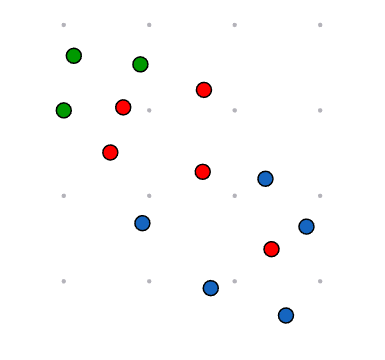
\includegraphics[width=0.8\textwidth]{images/lrus.png}

\end{figure}
\end{frame}

\begin{frame}{Limites des méthodes}
\begin{block}{SMOTE}
    \begin{itemize}
    \item Temps de calculs 
     \item Création de points aberrants
     \item Hyperparamètre k 
     \item Variables qualitatives
     \end{itemize} 
\end{block}
    
\end{frame}

\begin{frame}{Limites des méthodes}
\begin{block}{SMOTE}
    \begin{itemize}
       \item Points aberrants
   \end{itemize}  
\end{block}
    
    \begin{figure}
    \centering
    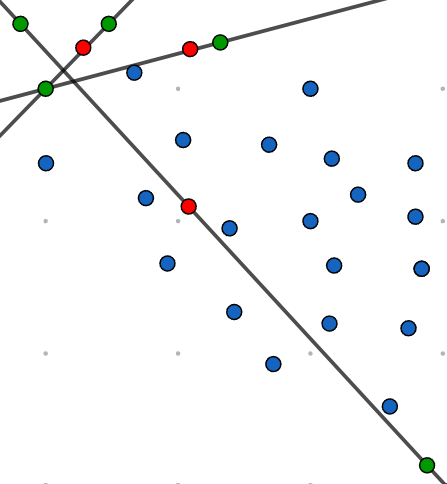
\includegraphics[width=0.5\textwidth]{images/lsmote.png}

\end{figure}
\end{frame}



\section{Application}

\begin{frame}

 \centering
\begin{tabular}{lcc}
\toprule
\textbf{Méthode} & \textbf{Transactions normales} & \textbf{Fraudes} \\
\midrule
ROS (Over-Sampling) & 284\,315 & 284\,315\\
RUS (Under-Sampling) & 492 & 492 \\
SMOTE & 284\,315 & 284\,315 \\
\bottomrule
\end{tabular}

\begin{block}{Comparaison des méthodes de rééchantillonnage (Régression Logistique)}
\centering
\begin{tabular}{lcccc}
\toprule
\textbf{Méthode} & \textbf{Accuracy} & \textbf{Recall} & \textbf{Balanced Accuracy} \\
\midrule
\textbf{RUS} & 0.956 & 0.959 & 0.956 \\
\textbf{ROS}  & 0.949 & 0.977 & 0.949 \\
\textbf{SMOTE} & 0.981 & 0.992 & 0.970 \\
\bottomrule
\end{tabular}
\end{block}

\end{frame}

\section{Conclusion}

\begin{frame}{Bilan général des méthodes}
    \centering
    \small
    \begin{tabular}{|l|p{3cm}|p{3cm}|}
        \hline
        \centering
        \textbf{Méthode} & \textbf{Points forts} & \textbf{Limites} \\
        \hline
        \centering
        ROS & Simplicité, conserve toutes les données & Overfitting, grand volume de données \\
        \hline
        \centering
        RUS & Rapide et réduit le biais & perte d'information et représentativité \\
        \hline
        \centering
        SMOTE & Données synthétiques variées & Coût élevé, sensible aux outliers \\
        \hline
    \end{tabular}
    \vspace{0.7cm}

    \textbf{Aucune méthode n’est universelle :}\\
    le choix dépend du jeu de données et du modèle.
\end{frame}

\begin{frame}{Conclusion et perspectives}
    \begin{itemize}
        \item Pour notre jeu de données, la méthode la plus efficace est SMOTE.\\[0.5cm]
        \item  Pour aller plus loin : il serait pertinent de combiner des méthodes existantes ou de pondérer les modèles.
    \end{itemize}
\end{frame}

\begin{frame}
    \centering
    \Huge Merci pour votre attention !
\end{frame}

\end{document}